\documentclass{beamer}
\usepackage{graphicx, amsmath, amssymb, textcomp}

\newcommand{\pyplot}{\includegraphics[width=\textwidth, trim=60px 60px 60px 40px]}
\renewcommand{\vec}{\mathbf}

\newcommand{\bottomcite}{\let\thefootnote\relax\footnote}

\let\oldfootnotesize\footnotesize
\renewcommand*{\footnotesize}{\oldfootnotesize\tiny}


\begin{document}

\setbeamertemplate{navigation symbols}{}

\title{Effectiveness of a superconducting lead endcap\\ in minimizing magnetic field gradients\\ for the nEDM search}
\author{Aritra Biswas\\Filippone Group, Kellogg Radiation Laboratory}
\maketitle

\begin{frame}
\frametitle{nEDM = neutron electric dipole moment}

    \begin{columns}

    \begin{column}{0.5\textwidth}
    \begin{itemize}
        \item up quark: $\frac{2}{3} e$
        \item each down quark: -$\frac{1}{3} e$
        \item electric dipole moment: vector measuring separation between + and - charges
              and their orientation
    \end{itemize}
    \end{column}
    
    \begin{column}{0.5\textwidth}
    \begin{figure}
    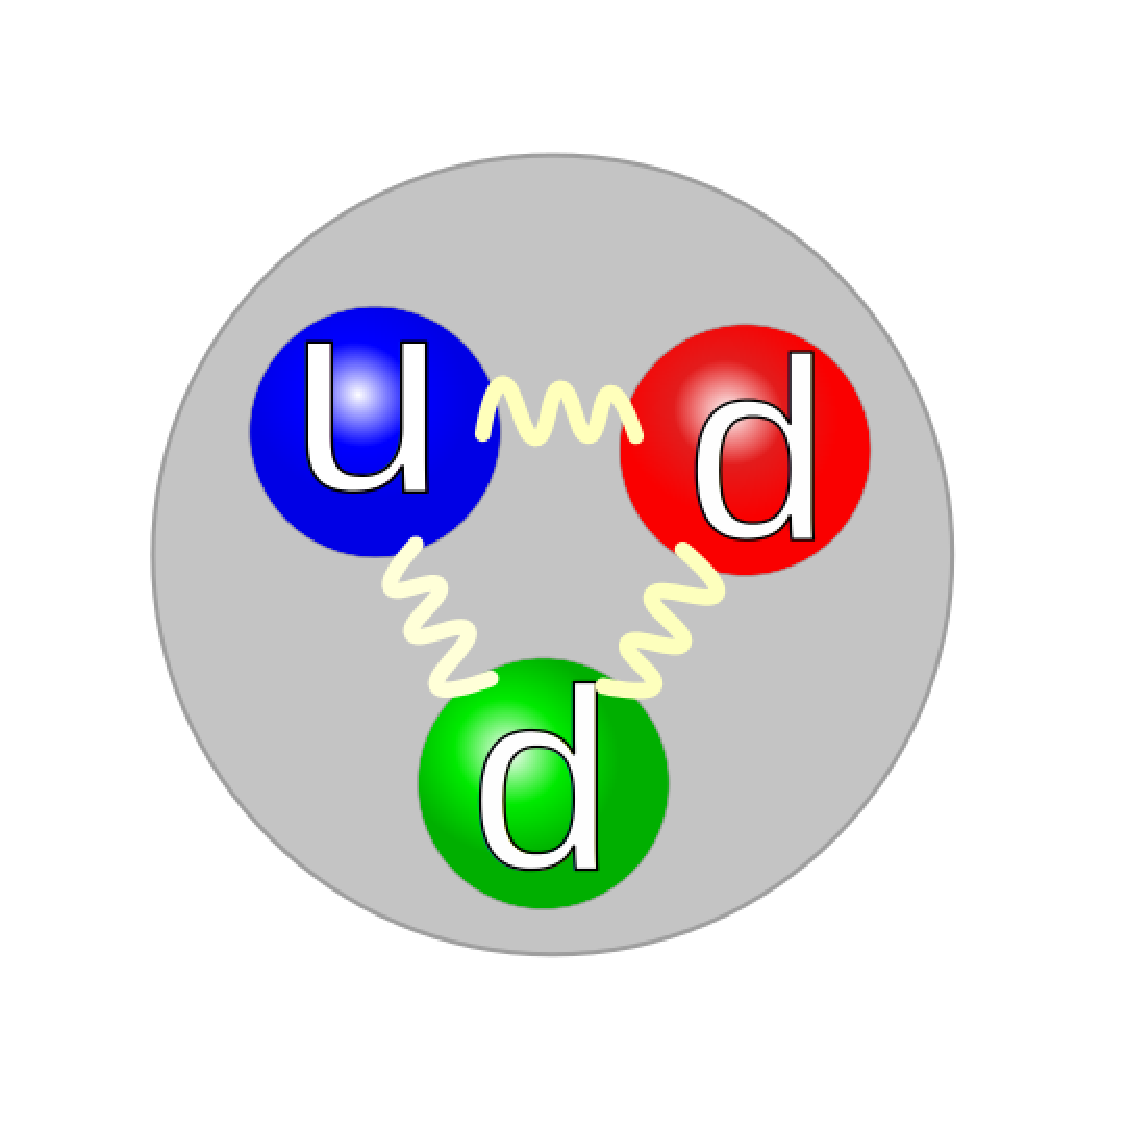
\includegraphics[width=\textwidth]{figures/neutron_quarks.eps}
    \end{figure}
    \end{column}

    \end{columns}

    \bottomcite{Horvath A. Quark structure neutron. Wikimedia.}

\end{frame}

\begin{frame}
\frametitle{why does the nEDM matter?}

    \begin{columns}
    
    \begin{column}{0.4\textwidth}
    \begin{figure}
    \includegraphics[width=\textwidth]{figures/nEDM_P_T_violation.png}
    \end{figure}
    \end{column}
   
    \begin{column}{0.6\textwidth}
    \begin{itemize}
        \item $C: q \mapsto -q$ \pause
        \item $P: (t, x, y, z) \mapsto (t, x, -y, z)$ \pause
        \item $T: (t, x, y, z) \mapsto (-t, x, y, z)$ \pause
        \bigskip
        \item $CPT$ symmetry \\\pause + $P$ violation \\\pause + $T$ violation \\
        \pause $\Rightarrow$ $CP$ violation \pause
        \bigskip
        \item reformulations of Standard Model
        \item matter-antimatter asymmetry
    \end{itemize}
    \end{column}

    \end{columns}
    
    \bottomcite{Knecht A. 22 May 2008. Parity and time reversal violation. Wikimedia. Public domain.}

\end{frame}

\begin{frame}
\frametitle{how do we measure the nEDM?}

    \begin{itemize}
        \item put ultra-cold neutrons (UCN) in $\vec{E}$ and $\vec{B}$ fields \pause
        \item neutron will precess at frequency $\omega$
        \begin{equation}
        \omega_{\uparrow\uparrow} = -\frac{\mu_n B + d_n E}{J\hbar}, \;\;\;
        \omega_{\uparrow\downarrow} = -\frac{\mu_n B - d_n E}{J\hbar}
        \end{equation} \pause
        \begin{equation}
        \Delta\omega = \pm\frac{2 \textcolor{blue}{d_n} E}{J\hbar} \pause \pm 
        \textcolor{red}{\Delta\omega_{geo}}
        \end{equation} \pause
        \item $\frac{\partial \vec{B}}{\partial (x,y,z)} \neq 0 \pause \Rightarrow
        \frac{\partial \vec{B}}{\partial t} \neq 0 \pause \Rightarrow$ effect of $\vec{E}$ field
        \pause
        $\Rightarrow \textcolor{red}{\Delta\omega_{geo}}$ \pause
        \bigskip
        \item geometric phase $\Rightarrow$ false measurement! 
    \end{itemize}

    \bottomcite{Pendlebury et. al. Geometric-phase-induced false electric dipole moment signals
    for particles in traps. Phys. Rev. A. 70, 032102 (2004).}

\end{frame}

\begin{frame}
\frametitle{creating an uniform magnetic field}

    \begin{columns}
    
    \begin{column}{0.5\textwidth}
    \begin{figure}
    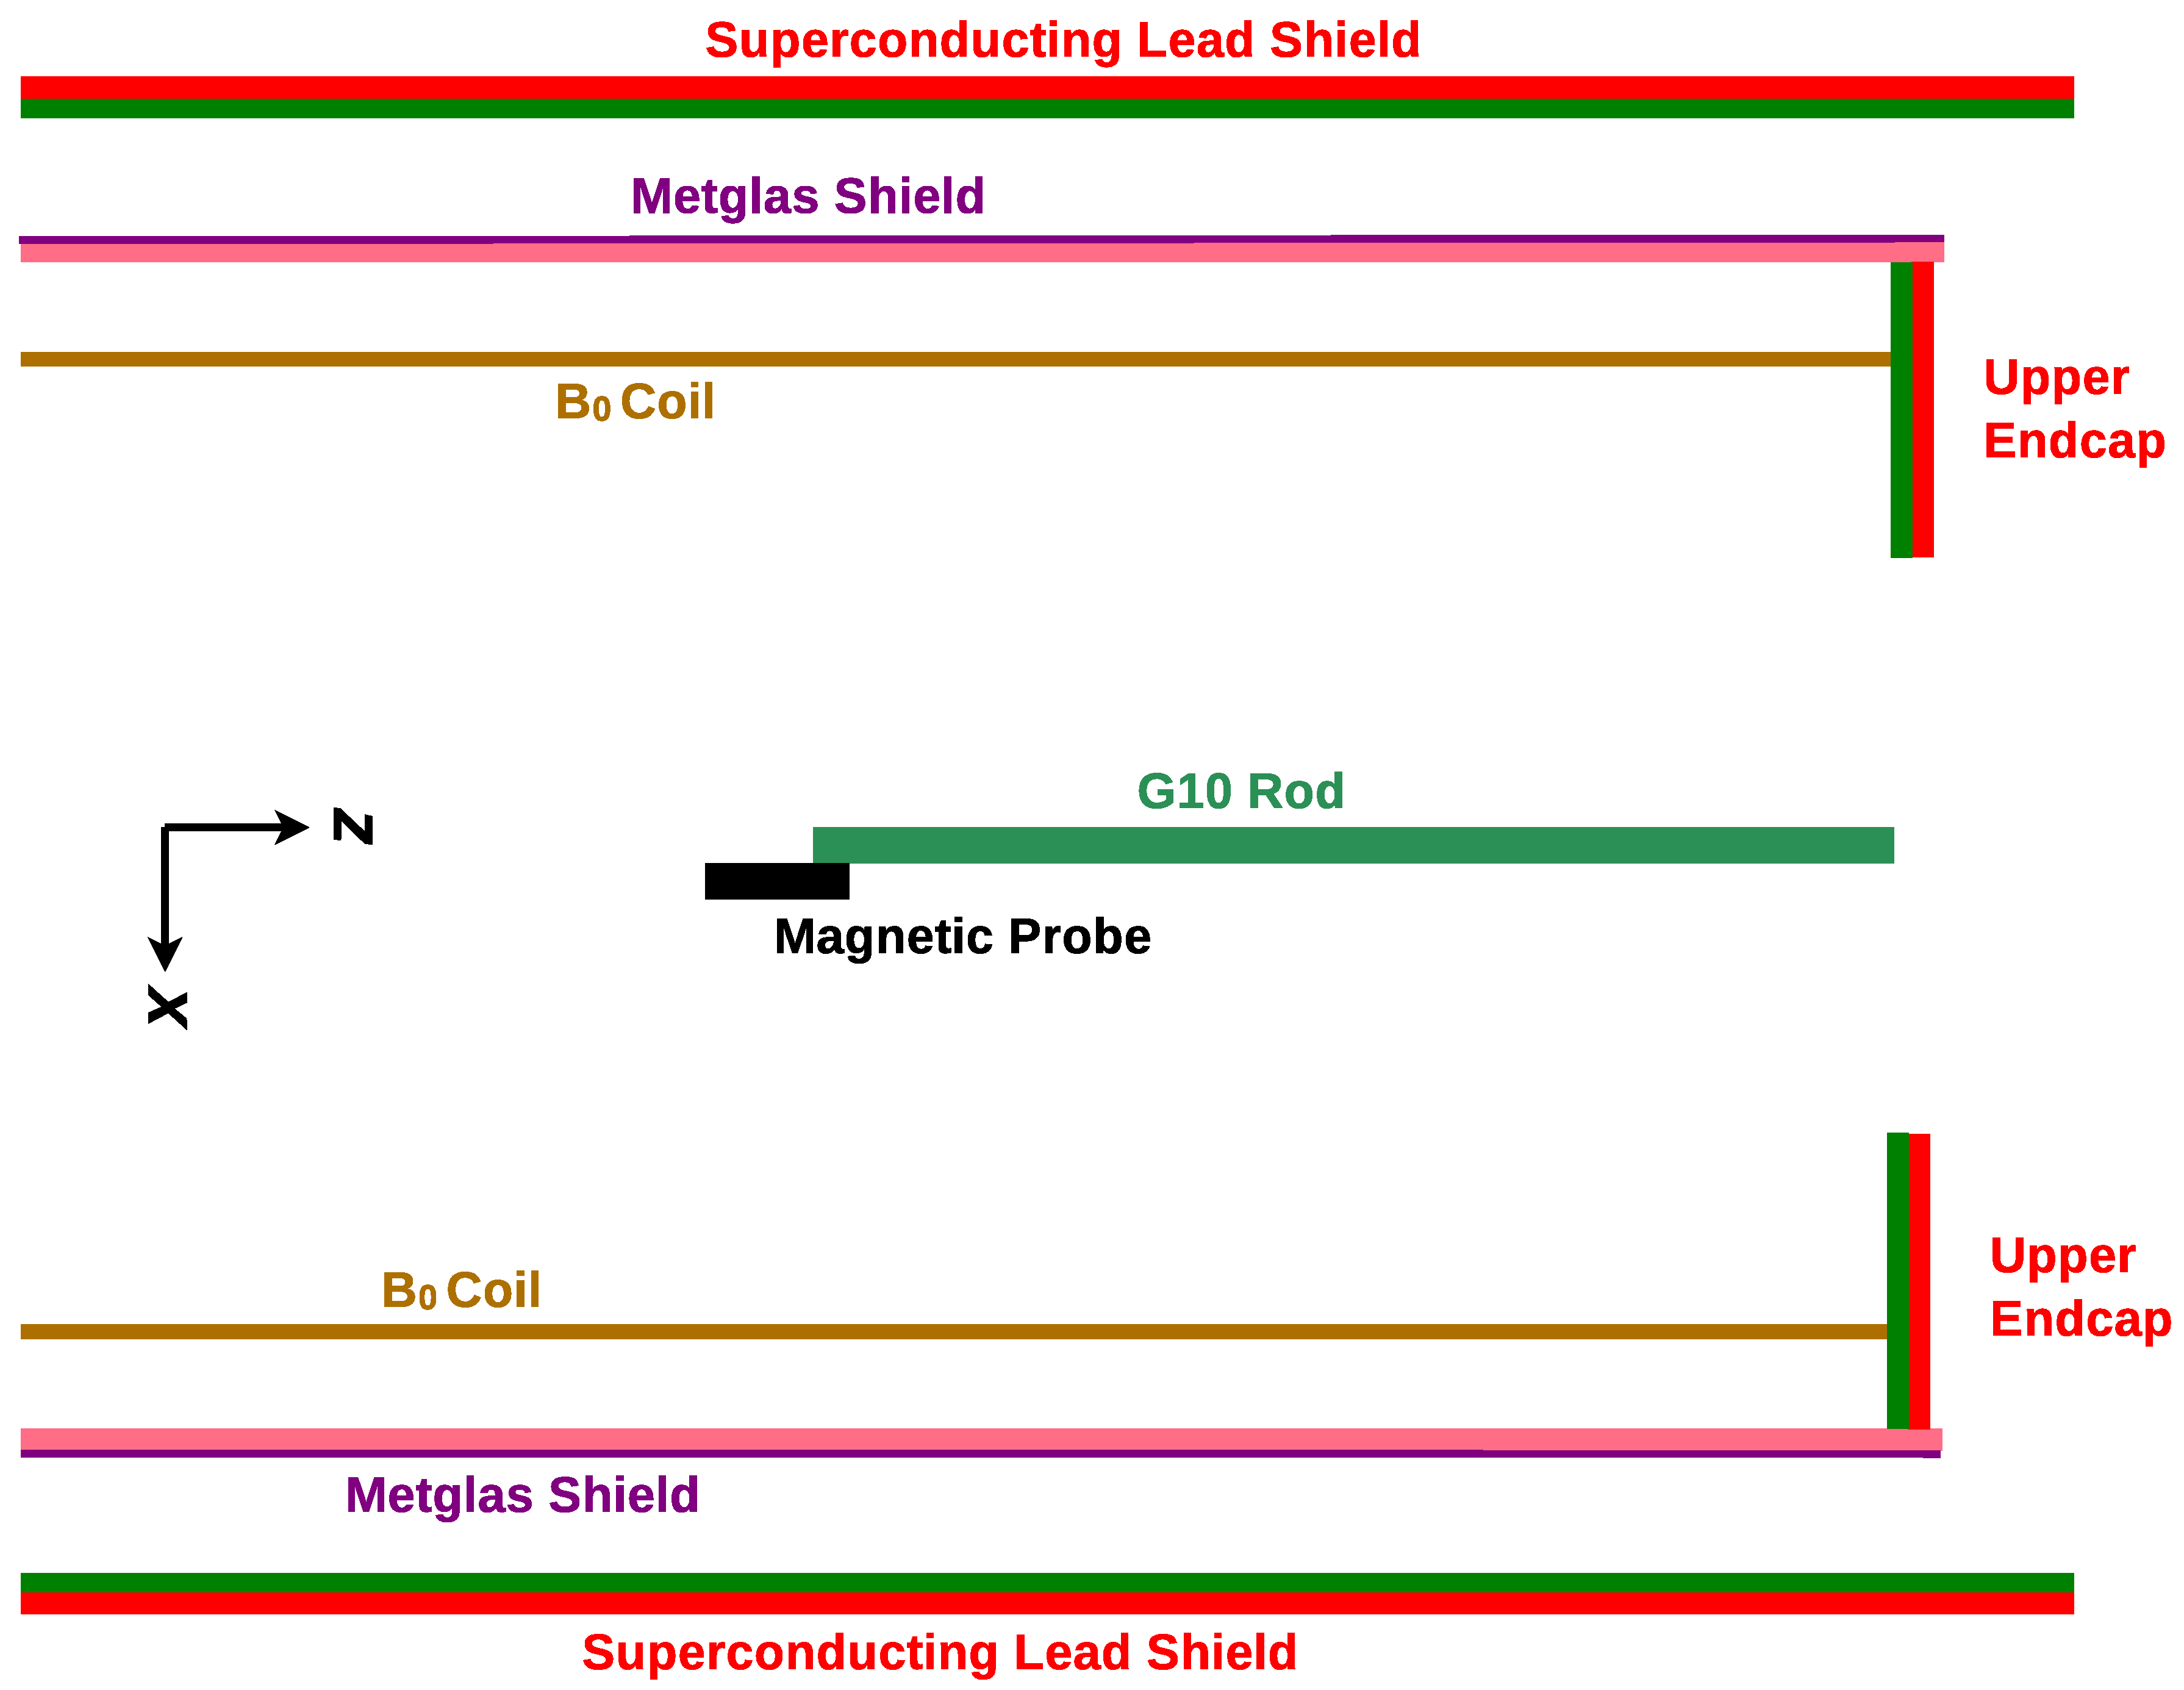
\includegraphics[width=\textwidth, angle=90, trim=70px 70px 70px 70px]
    {figures/simplified_structure.eps}
    \end{figure}
    \end{column}

    \pause

    \begin{column}{0.5\textwidth}
    \begin{itemize}
        \item $B_0$ coil: $\cos\theta$ coil geometry, emulates sheet current \pause
        \item ferromagnetic Metglas shield \pause
        \item superconducting axial shield \pause
        \item superconducting upper endcap
    \end{itemize}
    \end{column}

    \end{columns}

\end{frame}

%\begin{frame}
%\frametitle{analyzing the magnetic field profile}
%
%    \begin{itemize}
%        \item simulate experiment and calculate field
%        \item compare simulation and measurement in warm case
%        \item correct measurements
%        \item use simulation to predict effects of endcap
%        \item see whether measurements agree
%    \end{itemize}
%
%\end{frame}

\begin{frame}
\frametitle{original comparison, warm}

    \begin{center}
    \pyplot{../savedplots/original_Bz.eps}
    \end{center}

\end{frame}

\begin{frame}
\frametitle{Metglas thickness}

    \begin{center}
    \pyplot{../savedplots/thickness_Bz.eps}
    \end{center}

\end{frame}

\begin{frame}
\frametitle{Metglas 10 cm longer on top}

    \begin{center}
    \pyplot{../savedplots/longer10cm_Bz.eps}
    \end{center}

\end{frame}

\begin{frame}
\frametitle{correction 1: probe measurement time}

    \begin{center}
    \pyplot{../savedplots/upDown_Bz.eps}
    \end{center}

\end{frame}

\begin{frame}
\frametitle{correction 2: $x$ centering}

    \begin{center}
    \pyplot{../savedplots/manyx_Bz_z.eps}
    \end{center}

\end{frame}

\begin{frame}
\frametitle{correction 2: $x$ centering, superconducting}

    \begin{center}
    \pyplot{../savedplots/endcapOnAxis_dx0.eps}
    \end{center}

\end{frame}

\begin{frame}
\frametitle{correction 2: $x$ centering, superconducting, 1.4 cm offset}

    \begin{center}
    \pyplot{../savedplots/endcapOnAxis_dx1p4.eps}
    \end{center}

\end{frame}

\begin{frame}
\frametitle{comparison, superconducting}

    \begin{center}
    \pyplot{../savedplots/endcapOneBetter.eps}
    \end{center}

\end{frame}

%\begin{frame}
%\frametitle{comparison, superconducting}
%
%    \begin{center}
%    \pyplot{../savedplots/endcapThreeBetter.eps}
%    \end{center}
%
%\end{frame}

\begin{frame}
\frametitle{correction 3: probe axis offset}


    \begin{columns}
    
    \begin{column}{0.5\textwidth}
    \begin{figure}
    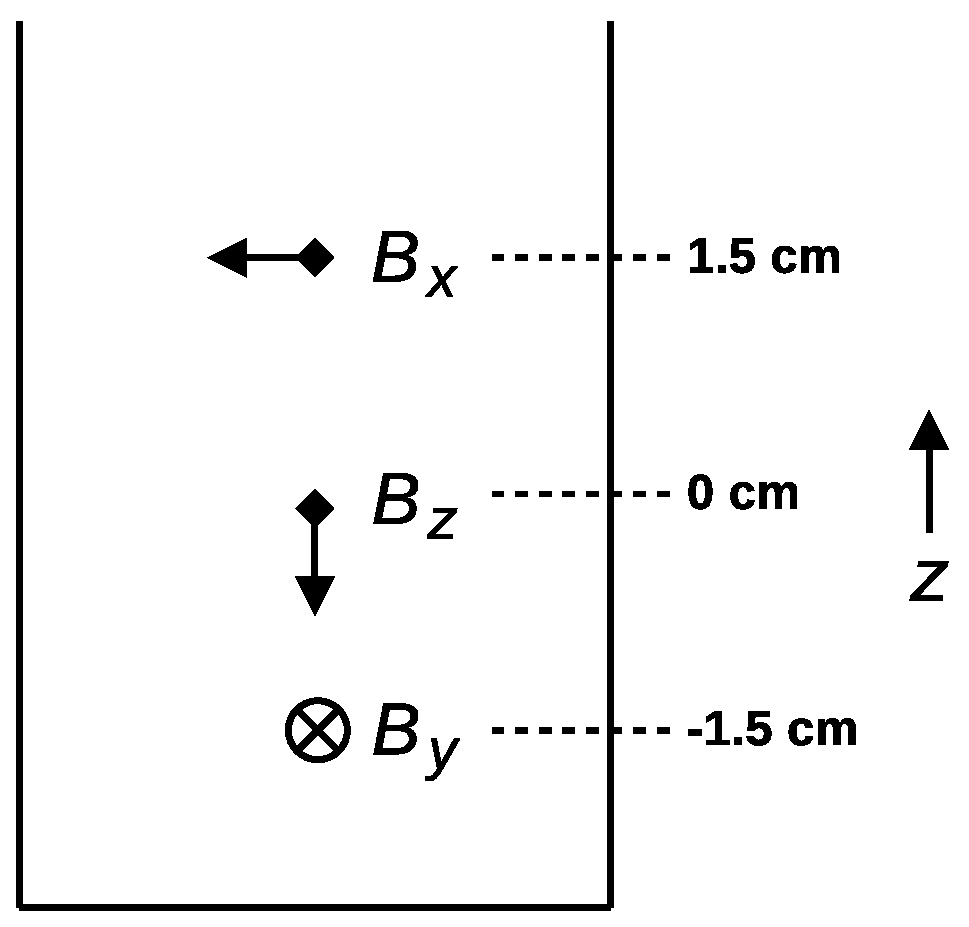
\includegraphics[width=\textwidth]
    {figures/probe.eps}
    \end{figure}
    \end{column}
    
    \begin{column}{0.5\textwidth}
    \begin{itemize}
        \item 3 separate 1-axis probes \pause
        \item incomplete vector map \pause
        \item need to store $z$-axis offset vector along with $z$ array \pause
        \item \texttt{OffsetAxis} class to return proper spatial axis array based
        on desired vector component
    \end{itemize}
    \end{column}
   

    \end{columns}

\end{frame}

\begin{frame}
\frametitle{comparison, superconducting, no offsets}

    \begin{center}
    \pyplot{../savedplots/endcapThreeNoOffset.eps}
    \end{center}

\end{frame}

\begin{frame}
\frametitle{comparison, superconducting, $x$-centering and axis offset}

    \begin{center}
    \pyplot{../savedplots/endcapThreeOffset.eps}
    \end{center}

\end{frame}

\begin{frame}
\frametitle{correction 4: probe tilt}
    
    \begin{center}
        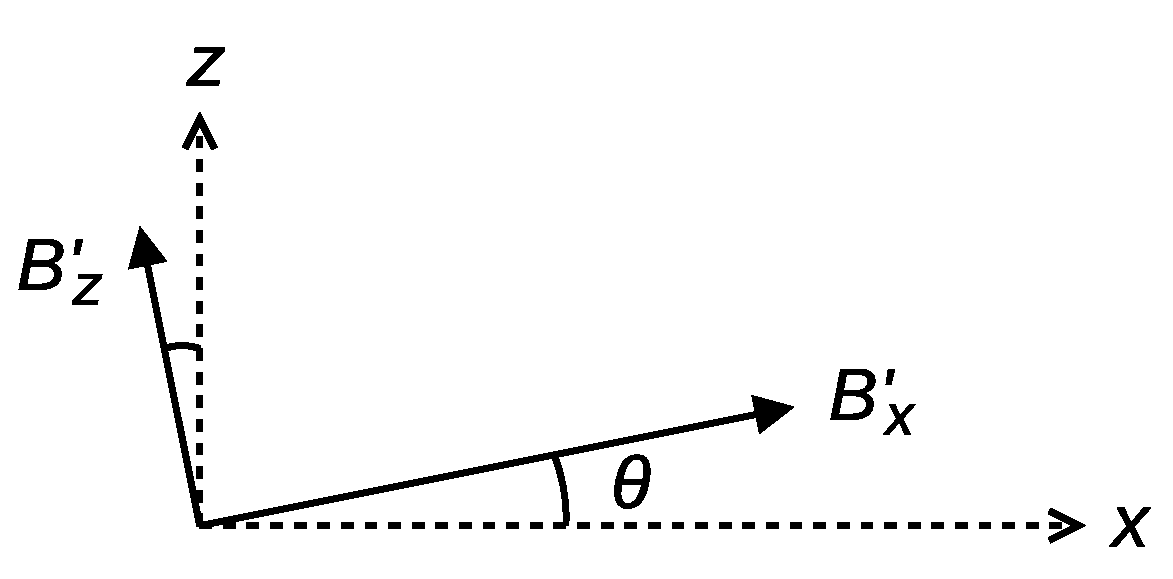
\includegraphics[width=0.5\textwidth]{figures/probe_tilt.eps}
    \end{center} \pause
    \begin{equation}
        B_x = B'_x \cos\theta - B'_z \sin\theta, \;\;\; B_z = B_z' \cos\theta + B_x' \sin\theta
    \end{equation}

    \pause

    \bigskip

    1. $\theta$ is small: \pause
    \begin{equation*}
        B_x = B'_x - B'_z \theta, \;\;\; B_z = B_z' + B_x' \theta
    \end{equation*} \pause
    2. $B_z = 0$ at center: \pause
    \begin{equation*}
        \theta = -\frac{B'_z}{B'_x}
    \end{equation*}

\end{frame}

\begin{frame}
\frametitle{comparison, superconducting}

    \begin{center}
    \pyplot{../savedplots/w5_comp.eps}
    \end{center}

\end{frame}

\end{document}
